\section{Experiments}
\label{sec:experiments}
{\renewcommand{\arraystretch}{1.05}
\begin{table}[t]
\centering
\small
\caption{\textbf{Results on General Agent Benchmarks.} We report accuracy (\%) on GAIA and FRAMES. \textbf{Bold} and \underline{underline} indicate best and runner-up results, respectively.}\label{tab:main1}
\vspace{1em}
\resizebox{0.96\linewidth}{!}{
\begin{tabular}{lcccccc}
    \toprule
    Method & Use idle? & GAIA Level1 & GAIA Level2 & GAIA Level3 & FRAMES & Average\\
    \midrule
    \multicolumn{7}{c}{\cellcolor[HTML]{E0E0E0}\textit{Gemma4-E4B}}\\
    \midrule
    Vanilla              & \xmark & 36.5$_{\pm 3.6}$ & 25.6$_{\pm 0.9}$ & \underline{11.5}$_{\pm 0.0}$ & 50.0$_{\pm 5.3}$ & 30.9\\
    +Sequential Revision & \xmark & 39.6$_{\pm 1.5}$ & \underline{26.4}$_{\pm 1.5}$ & 9.0$_{\pm 4.8}$ & \underline{53.3}$_{\pm 7.0}$ & \underline{32.1}\\
    +Sleep-time Compute  & \cmark & \underline{41.5}$_{\pm 4.1}$ & 23.6$_{\pm 3.8}$ & 9.0$_{\pm 4.8}$ & 50.0$_{\pm 5.3}$ & 31.0\\
    \midrule
    \rowcolor{green!10}
    \textbf{+ \methodname (Ours)} & \cmark & \textbf{43.4}$_{\pm 2.7}$ & \textbf{28.3}$_{\pm 2.1}$ & \textbf{14.1}$_{\pm 3.5}$ & \textbf{56.0}$_{\pm 3.5}$ & \textbf{35.5}\\
    \midrule
    \multicolumn{7}{c}{\cellcolor[HTML]{E0E0E0}\textit{Qwen3.5-4B}}\\
    \midrule
    Vanilla              & \xmark & 37.7$_{\pm 7.6}$ & 26.4$_{\pm 2.7}$ & \underline{11.5}$_{\pm 7.7}$ & \underline{57.3}$_{\pm 6.4}$ & 33.2\\
    \midrule
    +Sequential Revision & \xmark & \textbf{41.5}$_{\pm 5.0}$ & \underline{27.9}$_{\pm 3.1}$ & \underline{11.5}$_{\pm 7.7}$ & 56.0$_{\pm 4.0}$ & \underline{34.2}\\
    +Sleep-time Compute  & \cmark & 36.5$_{\pm 2.9}$ & 21.3$_{\pm 4.7}$ & 9.0$_{\pm 4.4}$ & 50.7$_{\pm 1.2}$ & 29.4\\
    \rowcolor{green!10}
    \textbf{+ \methodname (Ours)} & \cmark & \underline{40.9}$_{\pm 3.9}$ & \textbf{31.8}$_{\pm 3.6}$ & \textbf{21.8}$_{\pm 5.9}$ & \textbf{65.3}$_{\pm 4.2}$ & \textbf{40.0}\\
    \midrule
    \multicolumn{7}{c}{\cellcolor[HTML]{E0E0E0}\textit{Gemini-2.5-Flash}}\\
    \midrule
    Vanilla              & \xmark & 62.3$_{\pm 2.0}$ & 39.9$_{\pm 3.6}$ & \underline{25.6}$_{\pm 9.7}$ & 74.0$_{\pm 2.0}$ & 50.5\\
    \midrule
    +Sequential Revision & \xmark & 61.6$_{\pm 3.9}$ & 42.3$_{\pm 1.8}$ & 21.8$_{\pm 4.4}$ & \underline{76.7}$_{\pm 1.2}$ & \underline{50.6}\\
    +Sleep-time Compute  & \cmark & \underline{62.9}$_{\pm 2.9}$ & \underline{44.2}$_{\pm 2.0}$ & 20.5$_{\pm 5.9}$ & 72.7$_{\pm 1.2}$ & 50.1\\
    \rowcolor{green!10}
    \textbf{+ \methodname (Ours)} & \cmark & \textbf{66.0}$_{\pm 3.8}$ & \textbf{46.5}$_{\pm 4.2}$ & \textbf{32.1}$_{\pm 4.4}$ & \textbf{78.0}$_{\pm 4.0}$ & \textbf{55.6}\\
    \bottomrule
\end{tabular}}
\end{table}}
{\renewcommand{\arraystretch}{1.25}
\begin{table*}[t]
\centering
\small
\caption{\textbf{Results on MLE-Bench Lite.} 
We report the percentage of tasks that yield a submission, a valid submission, 
an above-median score, and each Kaggle medal tier (Bronze/Silver/Gold).
All methods are evaluated under the standard 24-hour wall-clock budget per task, using Gemini-2.5-Flash as the backbone. 
\textbf{Bold} and \underline{underline} indicate best and runner-up results, respectively.}
\label{tab:main2}
\resizebox{1.0\textwidth}{!}{
\begin{tabular}{lcccc cccc}
    \toprule
    \multirow{2}{*}{Method} & \multirow{2}{*}{Use idle?} &
    \multirow{2}{*}{\makecell{Made\\Submission\\(\%)}} &
    \multirow{2}{*}{\makecell{Valid\\Submission\\(\%)}} &
    \multirow{2}{*}{\makecell{Above\\Median\\(\%)}} &
    \multicolumn{4}{c}{Any Medal (\%)} \\
    \cmidrule(lr){6-9}
    & & & & & Bronze & Silver & Gold & Total \\
    \midrule
    Vanilla & \xmark &
    86.4 & 77.3 & 40.1 & 9.1 & 9.1 & 18.2 & 36.4 \\
    \midrule
    +Sequential Revision & \xmark &
    \underline{90.1} & \underline{81.8} & \underline{50.0} & 13.6 & 9.1 & 18.2 & \underline{40.9} \\

    +Sleep-time Compute & \cmark &
    \underline{90.1} & \underline{81.8} & \textbf{59.1} & 13.6 & 9.1 & 13.6 & 36.4 \\
    \rowcolor{green!10}
    \textbf{+ \methodname (Ours)} & \cmark &
    \textbf{95.5} & \textbf{86.4} & \textbf{59.1} & 13.6 & 13.6 & 18.2 & \textbf{45.5} \\
    \bottomrule
\end{tabular}
}
\end{table*}
}


We design experiments to answer the following questions:
\begin{itemize}[leftmargin=*,itemsep=0mm]
\item \textbf{RQ1:} Does \mname improve task performance on general agentic benchmarks (GAIA, FRAMES) across diverse LLM backbones? (Table~\ref{tab:main1} in Section~\ref{sec:main-results})
\item \textbf{RQ2:} Does \mname generalize to execution-heavy environments with substantial tool-execution times (MLE-Bench)? (Table~\ref{tab:main2} in Section~\ref{sec:main-results})
\item \textbf{RQ3:} How efficiently does \mname utilize idle time, is it compatible with other test-time scaling methods, and which design choices matter? (Figure~\ref{fig:latency-vs-acc} and Tables~\ref{tab:token-analysis}, \ref{tab:planning_composition}, \ref{tab:ultra-short-impact}, \ref{tab:ablation} in Section~\ref{sec:ablation})
\end{itemize}

\textbf{Datasets.}
We evaluate \mname on three benchmarks: GAIA~\cite{mialon2023gaia} (general agent, full 165-task validation split), FRAMES~\cite{krishna2024frames} (multi-hop QA, 50 samples), 
and MLE-Bench Lite~\cite{chan2024mle-bench} (ML engineering, 24-hour budget per task).

\textbf{Models.}
Our experiments primarily use the proprietary model Gemini-2.5-Flash.
In addition, we consider Gemma4-E4B and Qwen3.5-4B to validate \mname with recent small open-source models.

\textbf{Baselines.}
To evaluate the effect of idle-time utilization, we include a vanilla
baseline that performs no additional computation during idle time. Additionally, we include Sequential Revision \cite{zhu2025scaling}, which performs revision step after each new observation.
To compare against approaches that utilize idle time, we consider Sleep-Time Compute \cite{lin2025sleeptime}, which generates auxiliary contexts during idle periods via naive prompting and reuses them at test time.\footnote{More details including implementation details, evaluation protocols are provided in Appendix~\ref{sec:appendix_details}.}


\subsection{Main Results}\label{sec:main-results}

\textbf{Results on General Agent Benchmarks.}
We evaluate \methodname{} on the GAIA and FRAMES benchmarks, which involve a diverse tool suite (e.g., text and audio processing, search agents) to solve complex multi-hop reasoning problems.
As shown in Table~\ref{tab:main1}, \methodname{} consistently improves task success rates over all baselines across both benchmarks and across all three GAIA difficulty levels. \methodname{} achieves the highest average accuracy on every backbone, improving over Vanilla by 4.6\% on Gemma4-E4B (30.9 $\rightarrow$ 35.5), 6.8\% on Qwen3.5-4B (33.2 
$\rightarrow$ 40.0), and 5.1\% on Gemini-2.5-Flash (50.5
$\rightarrow$ 55.6). The gains are most pronounced on the harder Levels~2 and~3, suggesting that idle-time speculation is most beneficial when the underlying reasoning task is difficult.
In contrast, Sleep-Time Compute exhibits limited or inconsistent improvements and, in some cases, even degrades performance. In particular, this degradation is especially pronounced with smaller open-source models such as Qwen3.5-4B: because Sleep-Time Compute freely pre-generates auxiliary context based on assumed future queries, hallucinations introduced at this stage mislead subsequent reasoning. \methodname{} avoids this failure mode through dual drafting that covers both progressive and recovery scenarios, guiding the agent toward correct trajectories. We provide qualitative examples of both behaviors in Appendix~\ref{sec:appendix_qualitative}. 


\textbf{Results on MLE-Bench.} We further evaluate \methodname{} on MLE-Bench, which features long-horizon interactions and execution-heavy steps involving repeated code execution and model training. As shown in Table~\ref{tab:main2}, Sleep-Time Compute matches \methodname{} on the Above-Median metric but lowers the Gold-medal rate relative to Vanilla (13.6\% vs.\ 18.2\%) and yields no improvement in total medals --- consistent with our earlier observation that naively pre-generated context can mislead reasoning under observation uncertainty. In contrast, \methodname{} achieves the best results across nearly all metrics, raising the submission rate from 86.4\% to 95.5\%, the valid submission rate from 77.3\% to 86.4\%, and the overall medal rate from 36.4\% to 45.5\%, with consistent gains across Bronze, Silver, and Gold tiers.
Because MLE-Bench involves long-running tool calls such as model training, a non-trivial portion of the 24-hour wall-clock budget is otherwise spent waiting. \methodname{} converts this wasted idle time into useful LLM computation, generating diverse solution paths that translate into more valid submissions and more medal-tier solutions within the same time budget, highlighting that \methodname{} generalizes to execution-heavy agentic workloads.
\begin{figure*}[t]
\centering
\begin{minipage}[c]{0.42\linewidth}
\centering
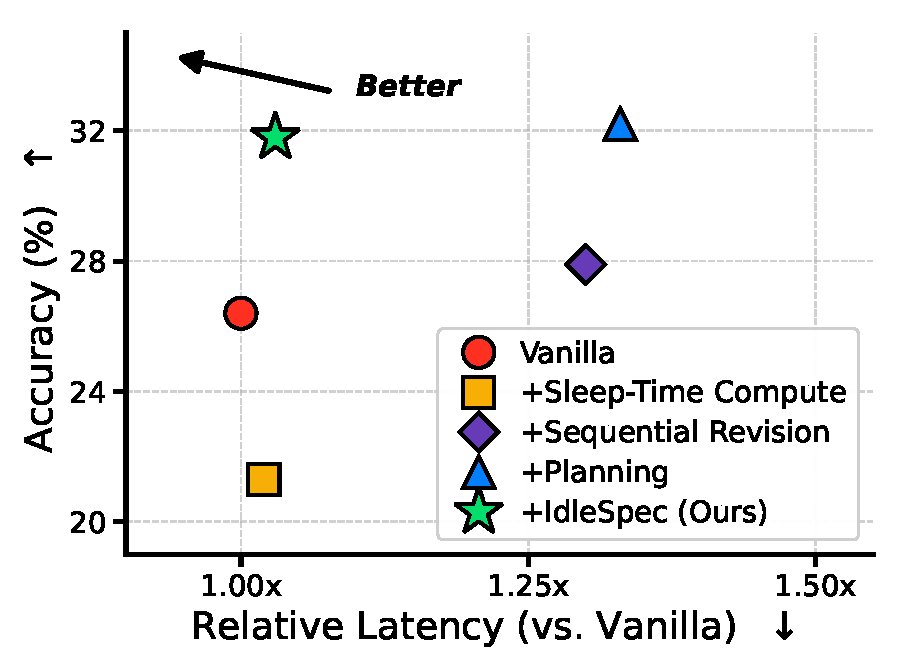
\includegraphics[width=\linewidth]{figures/latency_vs_acc.pdf}
\captionof{figure}{\textbf{Latency--Accuracy Trade-off.} All measurements were performed on vLLM using an NVIDIA A6000 GPU.}
\label{fig:latency-vs-acc}
\end{minipage}\hfill
\begin{minipage}[c]{0.55\linewidth}
\centering
\captionof{table}{\textbf{Idle-Time vs.\ Test-Time Token Usage.} Accuracy (\%) and output token usage during idle time and test time on GAIA Level 2 using Qwen3.5-4B.}
\label{tab:token-analysis}
\resizebox{\linewidth}{!}{
\begin{tabular}{lcc}
\toprule
Method & Accuracy & Tokens (Idle / Test)\\
\midrule
Vanilla              & 26.4 & (- / 7126)\\
\midrule
+Sequential Revision &  27.9 & (- / 11354)\\
+Planning        &  32.2 & (- / 12234)\\
+Sleep-time Compute & 21.3 & (3393 / 7048)\\
\rowcolor{green!10}
\textbf{+ \methodname (Ours)} & 31.8 & (5284 / 5966)\\
\bottomrule
\end{tabular}}
\end{minipage}
\end{figure*}


\subsection{More Analysis}\label{sec:ablation}
%We further analyze the effectiveness and efficiency of \methodname{} in utilizing idle time, its compatibility with existing test-time scaling methods, and the contribution of its individual design components.

\textbf{Efficiency Analysis.}
We analyze the efficiency of \methodname{} by comparing it against the original baselines (Sequential Revision and Sleep-Time Compute) and an additional test-time scaling baseline, \emph{Planning}, which generates a new plan after each tool-call observation before the next step.
As shown in Figure~\ref{fig:latency-vs-acc}, Sequential Revision and Planning improve accuracy by spending more tokens at test time, but this directly inflates end-to-end latency: Sequential Revision and Planning are about $1.30\times$ and $1.33\times$ slower than Vanilla, respectively.
\methodname{}, in contrast, achieves a Pareto improvement: it outperforms Sequential Revision and matches Planning's accuracy while keeping latency close to Vanilla, as most of its additional token computation is carried out during idle periods (Table~\ref{tab:token-analysis}).

\begin{table}[t]
\centering
\small
\setlength{\tabcolsep}{4pt}
\begin{minipage}[t]{0.45\linewidth}
\centering
\caption{\textbf{Compatibility with Test-Time Scaling.} Accuracy (\%) on GAIA Level~2 with Qwen3.5-4B. \methodname yields consistent gains when combined with existing test-time scaling methods. }
\label{tab:planning_composition}
\vspace{0.5em}
\begin{tabular}{lcc}
    \toprule
    Method & Use Idle? & Accuracy \\
    \midrule
    Sequential Revision  & \xmark & 27.9 \\
    \rowcolor{green!10}
    + \textbf{\methodname}  & \cmark & \textbf{32.2} \\
    \midrule
    Planning & \xmark & 32.2 \\
    \rowcolor{green!10}
    + \textbf{\methodname}  & \cmark  & \textbf{35.3} \\
    \bottomrule
\end{tabular}
\end{minipage}\hfill
\begin{minipage}[t]{0.45\linewidth}
\centering
\caption{\textbf{Effect of Idle-Time Length on Accuracy (\%).} GAIA samples are binned by their ultra-short ratio (the fraction of tool calls shorter than the reasoning step) with Gemini-2.5-Flash. Idle-time availability increases from High to Low.}
\label{tab:ultra-short-impact}
\vspace{1em}
\begin{tabular}{lccc}
    \toprule
    Method & High  & Medium  & Low \\
    \midrule
    Vanilla         & 50.0 & 39.0 & 39.0 \\
    \rowcolor{green!10}
    + \textbf{\mname} & 50.0 & \textbf{45.0} & \textbf{46.0} \\
    \bottomrule
\end{tabular}
\end{minipage}
\end{table}

\textbf{Compatibility with Test-Time Scaling.}
We investigate whether \methodname{} is complementary to existing test-time scaling methods, under the hypothesis that the two operate along orthogonal axes and can be seamlessly combined: \methodname{} scales computation along the \emph{idle-time} axis, while existing test-time scaling methods scale along the \emph{test-time} axis.
Since \methodname{} leaves the test-time procedure itself untouched, it can be layered on top of any such method without modification.
To verify this, we combine \methodname{} with the two test-time scaling baselines introduced above Sequential Revision and Planning,  while leaving each baseline's test-time procedure unchanged. As shown in Table~\ref{tab:planning_composition}, \methodname{} yields consistent gains on top of both baselines, improving Sequential Revision from 27.9\% to 32.2\% and Planning from 32.2\% to 35.3\%.
This gain likely arises because the progressive and recovery drafts generated during idle periods pre-expand the search space available at test time, which the test-time scaling method leverages to produce better-informed revisions and plan updates.

\textbf{Effect of Idle-Time Length.}
We analyze how the available idle time per step affects \methodname{}.
We define the \emph{ultra-short ratio} of a sample as the fraction of its tool calls whose execution time is shorter than a single LLM reasoning step. On GAIA, this ratio averages 25--27\% across the three difficulty levels (Appendix~\ref{sec:appendix_idle_length}, Table~\ref{tab:ultra-short-ratio}), indicating that most tool calls leave enough idle time for speculative drafting. Binning GAIA samples by ultra-short ratio into High (>0.75, least idle time), Medium (0.25--0.75), and Low (<0.25, most idle time) groups (Table~\ref{tab:ultra-short-impact}), we find that \methodname{} matches the vanilla baseline on the High group, where little usable idle time is available,  but delivers gains of 6.0 \% and 7.0 \% on the Medium and Low groups, respectively.

\begin{table}[t]
\centering
\small
\caption{\textbf{Ablation Studies.} Accuracy (\%) on GAIA and FRAMES when selectively ablating individual components of \methodname. (a) Drafting strategy on GAIA Level 1--3 using Gemini-2.5-Flash; (b, c) aggregation and selection strategies on FRAMES using Qwen3.5-4B.}
\label{tab:ablation}

\begin{subtable}[t]{0.40\linewidth}
\centering
\caption{Drafting Strategy}\label{tab:strategy}
\small
\setlength{\tabcolsep}{4pt}
\begin{tabular}{cccccc}
    \toprule
    Prog. & Rec. & L1 & L2 & L3 & Avg.\\
    \midrule
    \cmark & \xmark & 62.9 & 44.2 & 26.9 & 44.7\\
    \xmark & \cmark & 60.4 & 43.4 & 28.2 & 44.0\\
    \rowcolor{green!10}
    \cmark & \cmark & \textbf{66.0} & \textbf{46.5} & \textbf{32.1} & \textbf{48.2}\\
    \bottomrule
\end{tabular}
\end{subtable}\hspace{0.5em}
\begin{subtable}[t]{0.24\linewidth}
\centering
\caption{Aggregation}\label{tab:aggregation}
\small
\setlength{\tabcolsep}{4pt}
\begin{tabular}{lc}
    \toprule
    Method & Acc. \\
    \midrule
    Best-of-N & 59.3 \\
    Mandatory & 57.3 \\
    \rowcolor{green!10}
    \textbf{Ref. (Ours)} & \textbf{65.3} \\
    \bottomrule
\end{tabular}
\end{subtable}\hspace{0.5em}
\begin{subtable}[t]{0.24\linewidth}
\centering
\caption{Selection}\label{tab:selection}
\small
\setlength{\tabcolsep}{4pt}
\begin{tabular}{lc}
    \toprule
    Method & Acc. \\
    \midrule
    Random & 63.3 \\
    Forecast-Direct & 60.7 \\
    \rowcolor{green!10}
    \textbf{Adapt. (Ours)} & \textbf{65.3} \\
    \bottomrule
\end{tabular}
\end{subtable}
\end{table}

\textbf{Ablation Study.}
We ablate the three key design choices of \methodname{} --- drafting strategy, aggregation scheme, and selection rule.
First, Table~\ref{tab:strategy} shows that using only progressive or only recovery drafts underperforms, with recovery-only being especially harmful as the agent keeps switching plans without sufficient forward progress; sampling between the two yields the best results by balancing exploitation and exploration.
Second, Table~\ref{tab:aggregation} shows that simple aggregation schemes such as \emph{Best-of-N} (selecting a single plan) and \emph{Mandatory Selection} (enforcing all drafted plans) yield limited gains, whereas treating draft candidates as \emph{references} rather than strict constraints significantly improves accuracy.
Third, Table~\ref{tab:selection} shows that other selection rules (Random and Forecast-Direct) underperform, while the proposed adaptive selection achieves the highest accuracy.
